\chapter{ĐƠN HÌNH}

\section{Đơn hình chuẩn}
\indent Mỗi hình xuyến, mặt phẳng xạ ảnh ,bằng cách xác định các cạnh đối diện được chỉ ra bởi các vecto :
\begin{figure}[h]  
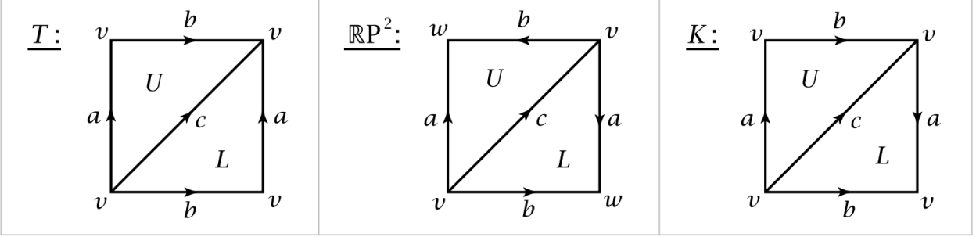
\includegraphics[width=\textwidth]{figures/chap1_1_1}
\caption[Cạnh đối diện vecto]{Cạnh đối diện vecto
\label{fig:chap1_1_1}}
\end{figure}

\indent Cắt một hình vuông theo một đường chéo sẽ tạo ra hai hình tam giác, vì vậy mỗi bề mặt này cũng có thể được dựng từ hai tam giác bằng cách xác định các cạnh của chúng theo từng cặp. Tương với một đa giác ,với bất kỳ số cạnh nào cũng có thể được cắt dọc đường chéo thành  hình tam giác. Như vậy, với đơn hình chuẩn \(n\) chiều  ∆n , dễ dàng thấy  ∆0 là một điểm, ∆1 là một đoạn thẳng, ∆2 là một tam giác, ∆3 là một tứ diện,...

\begin{figure}  
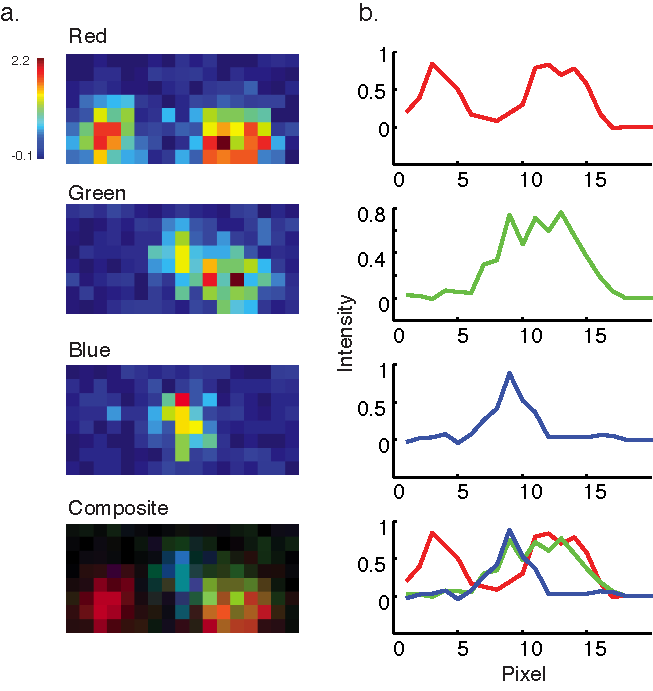
\includegraphics[width=\textwidth]{figures/fullpage}
\caption[Short figure name.]{This is a full page figure using the FPfigure command. It takes up the whole page and the caption appears on the preceding page. Its useful for large figures. Harvard's rules about full page figures are tricky, but you don't have to worry about it because we took care of it for you. For example, the full figure is supposed to have a title in the same style as the caption but without the actual caption. The caption is supposed to appear alone on the preceding page with no other text. You do't have to worry about any of that. We have modified the fltpage package to make it work. This is a lengthy caption and it clearly would not fit on the same page as the figure. Note that you should only use the FPfigure command in instances where the figure really is too large. If the figure is small enough to fit by the caption than it does not produce the desired effect. Good luck with your thesis. I have to keep writing this to make the caption really long. LaTex is a lot of fun. You will enjoy working with it. Good luck on your post doctoral life! I am looking forward to mine. \label{fig:myFullPageFigure}}
\end{figure}
\afterpage{\clearpage}


\section{This is section two}
\blindtext
\blindmathpaper

\section{This is section three}
\blindtext
\blindmathpaper